\documentclass{article}
\usepackage{graphicx}
\usepackage[nottoc,numbib]{tocbibind}
\usepackage[a4paper, total={6in, 8in}]{geometry}
\usepackage{subcaption}
\newcommand{\myparagraph}[1]{\paragraph{#1}\mbox{}\\}
 
\usepackage{xcolor}
\newcommand{\highlight}[1]{\colorbox{yellow!50}{$\displaystyle#1$}}


\title{Machine Learning \& Applications\\Open Assessment}
\author{Y1481702}
\date{\today}
\setlength\parindent{0pt}
 
\begin{document}
 
\begin{titlepage}
\maketitle
\tableofcontents
\end{titlepage}
 
\section{The Expectation-Maximisation Algorithm}
\subsection{Task 1}
\myparagraph{Program } %[5 Marks] - IT WORKS!
\texttt{mlap\textunderscore prog 1 task1.dat}


\myparagraph{Explain how the maximum likelihood estimates (MLEs) have been computed.} %  Max 50 words. [5 Marks]
These maximum likelihood estimates (MLEs) have been found by counting the occurrence of each property value and dividing this by the total number of data points for that property. This can be used as an estimate of the probability distribution for the given property.\\

\textit{NB. Given the small sample size, the MLEs may not accurately reflect the true probabilities of the distribution, if the size of the sample data, n, is increased, they would become increasingly correct as $n \to \infty$.}

\subsection{Task 2}
\myparagraph{Program} %[12 Marks] - It Works
\texttt{mlap\textunderscore prog 2 task2.dat}

\myparagraph{Explain how the EM has been implemented.}
% Max 150 words. [8 Marks]
The Baum-Welch instance of the EM algorithm has been implemented using Python. To allow code reuse between tasks, each task instantiates a new \texttt{EMAlgorithm} object with the necessary distribution parameters. Each iteration of the algorithm consists of three steps, computing the forward probabilities, computing the backward probabilities, before finally computing an updated model of the distribution. The forward step calculates the probabilities of the robot being in each square at a given time. The backward step determines the probabilities that the given emission sequence has occurred at each time given a particular starting cell. Finally the original distributions can be updated with increasingly likely values using Bayes theorem and the probabilities calculated in the previous two steps. In this case, these steps are run iteratively until the log-likelihood change between iterations becomes less than 0.01, as specified by the requirements. Iterating any further than this could risk over-fitting the distributions to our training data set.

\subsection{Task 3}
\myparagraph{Program} % [5 Marks] - no luck so far...
\texttt{mlap\textunderscore prog 3 task2.dat}

\myparagraph{Explain why different log-likelihoods are achieved for different EM runs.}
% (You should get different behaviour with random initialisation than with the uniform initialisation in Task 2.) Max 200 words. [5 Marks]
The random initialisation of the input distributions for initialisation, transition and emission properties add a significant non-deterministic component into the result. With each iteration, these randomly initialised distributions are moved in the direction of increasing maximum likelihood estimate for the parameters of the hidden Markov model. Rather than guarantee a global maximum, which would take far longer to compute, the algorithm finds the distribution with local maximum likelihood. Intuitively, if the distributions start from a different random location on each run, they may find a different local maximum each time.

\subsection{Task 4}
\myparagraph{Program} % [5 Marks] not started?
\texttt{mlap\textunderscore prog 4 task2.dat}

\myparagraph{Explain how the EM algorithm has been altered to use the information specified.} % Max 200 words. [5 Marks]
The input distributions ($\lambda = (A, B, \pi)$) have been set accordingly for the information that is known about the problem. Specifically, in the transition distribution $A$, a probability of 0 is given in the case where the robot between two given cells, either due to a wall or the cells not being adjacent. All other transitions are initialised randomly, such that the distribution sums to 1. During the forward step of the algorithm, the probabilities of being in a particular cell at a given time will be computed using this input transition distribution.
\[\alpha_j(t+1) = B_j(y_{t+1}) \sum_{i=1}^{N}\alpha_i(t)\highlight{A_{ij}}\]
Clearly if the transition is not possible, the value of $A_{ij}$ will be 0 and hence the result of the whole $\alpha_j(t+1)$ term will be 0. This value is passed further through the iteration as a product in the temporary variable $\xi$, and back into the updated value of $A$. 
\[\xi = \frac{\highlight{\alpha_i(t)}\highlight{a_{ij}}\beta_j(t+1) b_j(y_{t+1})}{\sum_{i=1}^{N}\sum_{j=1}^{N} \alpha_i(t) a_{ij} \beta_j(t+1)b_j(y_{t+1})}\]
\[a_{ij} = \frac{\sum_{t = 1}^{T-1}\highlight{\xi_{ij}(t)}}{\sum_{t = 1}^{T-1}\gamma_i(t)}\]
As such, when the algorithm iterates, the values that have been given will be resilient through to the updated transition distribution. Hence, no additional alterations are needed to ensure the algorithm makes full use of all the information known about the given problem.

\newpage
\section{Manifold Learning}
\subsection{Introduction}
It is often the case with high dimensional data that all samples lie upon a lower dimensional manifold within the available Euclidean data-space. This can be impossible to visualise once the data becomes represented by more than three dimensions, but Figure \ref{fig:swiss-roll} shows a classic example of this where data lies upon a two dimensional `swiss roll' manifold in three dimensional space. Isomap, Laplacian Eigenmaps (LE) and Locality Preserving Projects (LPP), as proposed by \cite{isomap, le, lpp} respectively, are three available algorithms for projecting the manifold into the lesser number of dimensions with minimal loss of data. This allows the data points to be plotted in the minimal number of dimensions of true variance, allowing simpler and more efficient processing, for use in various applications, including facial recognition.

\subsection{In qualitative terms, describe how each algorithm works.}
%Without using mathematics, in qualitative terms describe how each algorithm works. Use diagrams where they help to explain your answer. [10 Marks]
\subsubsection{Isomap}
Isomap aims to combine the computational efficiency, global optimality and asymptotic convergence of PCA and Multi-Dimensional Scaling (MDS) with the flexibility to learn a broad class of non-linear manifolds\cite{isomap}. In layman's terms, the algorithm creates a graph (Fig \ref{fig:k-nearest-neighbours}), only connecting data points which are closest to each other and then calculates the distance of the shortest route from one point to another traversing through these connections only (Fig. \ref{fig:route}). After this, it runs classical MDS to map out the points from these distances.

\subsubsection{Laplacian Eigenmap}
The data-proximity graph is computed in the same way as isomap, described above. This graph gives an estimation for the data manifold. The algorithm then computes the Laplacian of the graph. As the Laplacian matrix is square, symmetric and positive semidefinite, we can find its eigendecomposition. This decomposition gives us the eigenvectors and eigenvalues of the matrix which represents the data. Any zero-valued eigenvalues, of which there should be at least one, have a corresponding eigenvector which relates to a dimension in the dataset that will be discarded.

\subsubsection{Locality Preserving Projection}%Locality Preserving Projections, as the name would suggest, attempts to preserve the neighbourhood structure of the dataset. But so do ALL the methods..
Once again, in order for the algorithm to estimate the data manifold, the data proximity graph is computed as described above. This algorithm then uses the Laplacian of this graph to compute a transformation matrix which can be used to map each of the original data points into the desired lower dimensional space. Unlike isomap and Laplacian Eigenmap, LPP creates a full mapping from the original data-space to the lower-dimensional one, rather than simply transforming the given data. This means the transformation matrix can be used on any data point that falls within the original space, including unseen data. As such, it may also be useful for classification problems because it can be used to reduce the dimensionality of unseen data even after the projection has been initially calculated using a training data set. LPP is linear reduction like principle components analysis (PCA). This means it is faster to compute for larger datasets potentially making it be more useful in practice\cite{lpp}. However, as shown by Fig. \ref{fig:isomap} its lineality means it may not be able to ideally map the manifold. Additionally, because of it's locality preserving nature, LPP has more discriminating power than PCA and is less sensitive to outliers.

\subsection{Explain the role of the data proximity graph.}
%The methods each utilise a data proximity graph at some stage. Explain the different role of the graph in the three methods. [5 Marks]
All three methods use the graph to determine whether two particular data points preside on the same manifold, i.e. are connected, directly or indirectly, in the data proximity graph. This graph is key to learning the structure of the manifold that the data lies upon. As can be clearly seen from Fig. \ref{fig:k-nearest-neighbours}, if the graph is constructed correctly the manifold can be effectively captured by it- it is an approximation of the manifold. Each method generates a new matrix from the data proximity graph. In each of these matrices the columns and rows each represent each data point in the sample, hence each element in the matrix corresponds to two specific data points.\\

In Step 2 of the isomap algorithm this new matrix is created using the data proximity graph. The matrix values represent the shortest distance between the respective two data points on the graph (Fig. \ref{fig:route}). As the graph is an approximation of the manifold, this distance value is itself an approximation of the distance between the points travelling along the data manifold. If the corresponding vertices on the graph are not connected (either directly or indirectly) they do not exist on the same manifold, in which case the matrix element will be set to positive infinity.\\

\label{weights-matrix}
The matrix created by both LPP \& LE contains values calculated as $W_{ij} = e^{-\frac{\left|\left|\vec{x_i} - \vec{x_j}\right|\right|^{2}}{t}}$. Unlike the isomap matrix, values will be calculated only for nodes which are directly connected. Any matrix elements where the data points aren't connected are set to 0.

\subsection{Describe how the Laplacian matrix is constructed.}
%One of the mathematical tools used in these methods is the Laplacian matrix. Describe how this matrix is constructed from a graph, and explain the significance of the Fiedler vector. [5 Marks]
\label{laplacian-matrix}
The Laplacian matrix $L$ is a positive, semidefinite matrix that can be though of as an operator on functions defined on vertices of the data proximity graph, $G$, and is defined as
\[L = D - W\]
where $W$ is the symmetric matrix of weights created by the LPP \& LE algorithms, as described in Section \ref{weights-matrix} above, and D is a diagonal matrix, created from W, where each element ($D_{ii}$) is the sum of the row (and column) of its corresponding element in W ($W_{ii}$)\cite{le}. 
$$D_{ii} = \sum_{j=0}^{N} W_{ji} = \sum_{i=0}^{N} W_{ji}$$
The Laplacian matrix of a graph is particularly useful as it is always square, positive and semidefinite which means it will always be eigendecomposible with $N$ eigenvectors.


\subsection{Explain the significance of the Fiedler vector.}
The Fiedler vector of the data proximity graph, first proposed in 1973\cite{fiedler_1973}, is the second smallest eigenvalue, $\lambda_{n-2}$, of the Laplacian Matrix $L$. The Laplacian matrix will have an eigenvalue equal to 0 for each connected component in the data proximity graph it has been calculated from. As such, if the Fiedler vector is greater than 0, it is a full connected graph.\\

\label{data-prox-types}
The Fiedler value will be greater in magnitude for a more connected graph, which gives useful applications. Again, this can be particularly useful in the analysis of the data proximity graph. If the Fiedler vector value is unexpectedly high it may point to short-circuit errors between layers in the curved manifold, if it is too low, this may indicate a fragmented manifold with a large number of disconnected regions\cite{isomap_stability}. As such, it may help decide if the data proximity needs to be calculated again using a value, for either k-nearest neighbours or for $\epsilon$-neighbourhoods, that has been adjusted up or down. More recently this has also been applied in other fields, such as analysing network robustness\cite{fiedler_networks, fiedler_networks2}.

\subsection{Give a brief mathematical description of each algorithm.}
% For each of the methods in turn, give a brief mathematical description of the algorithm, commencing from $X$. [15 Marks]
Suppose you are given a set of data $X = {\vec{x_1}, ..., \vec{x_N}}$ where $\vec{x_i}$ is the i\textsuperscript{th} vector which is of length $d$ and there are $N$ such vectors. The aim is to produce a new set of data $Y = {\vec{y_1}, ..., \vec{y_N}}$ where $\vec{y_i}$ is the i\textsuperscript{th} vector which is of length $c \bullet c \leq d$, such that $Y$ more accurately represents the intrinsic dimensionality of that data. Each algorithm begins by generating a data proximity graph for $X$.\\

\subsubsection{Data Proximity Graph}
There are two methods of generating the data proximity graph, $k$-nearest neighbours or $\epsilon$-neighbourhoods. In each method, this value for either $k$ or $\epsilon$ is the only free parameter that must be determined. It is important to ensure the value of this parameter is appropriate for the data domain, as discussed in Section \ref{data-prox-types}. The resulting data proximity graph will have $N$ nodes, connected by a set of edges, $E$. These edges will, if successful, lie along the manifold that is being modelled.\\

In the k-Nearest neighbours method, nodes $i$ and $j$ are connected by an edge, $e$, if $j$ is one of the $k$ closest nodes to $i$:
\[ \forall i, j \in X \bullet i \ne j \land j \in \mathrm{nearest}(i, k) \land i \in \mathrm{nearest}(j, k) \Leftrightarrow \exists e \in E \bullet e = \{i, j\} \]
where nearest($\vec{x_i}$, $k$) returns the set of k elements that are closest to $\vec{x_i}$ in the Euclidean data-space.\\

Alternatively, using $\epsilon$-neighbourhoods, an edge, $e$, is added if the Euclidean distance between two nodes is less than a given value of $\epsilon$:
\[ \forall i, j \in X \bullet i \ne j \land \left|\left|\vec{x_1} - \vec{x_2}\right|\right|^2 < \epsilon \Leftrightarrow \exists e \in E \bullet e = \{i, j\} \]

Each of the algorithms then use different methods for setting the weights of the edges, $E$ in the graph.

\subsubsection{Isomap}
In the isomap method, the weights of each edge in the graph is set to the distance between $i$ and $j$ in the high-dimensional input-space. This distance ($\mathrm{d}(i, j)$) can be measured either by standard Euclidean distance ($\mathrm{d}(i, j) = \left|i - j\right|$), or alternatively, by some domain specific metric.
\[\forall i,j \in X \bullet (\exists e \in E \land e = \{i, j\}) \Leftrightarrow \mathrm{w}(e) = \mathrm{d}(i, j) \]

The second stage of isomap produces an $N \times N$ matrix $M$, such that:
\[M_{ab} = \left\{
\begin{array}{ll}
      \mathrm{d}(a, b) & \exists e \in E \bullet e = \{a, b\} \\
      \mathrm{d}(a, F_1) + \sum_{i = 1}^{\left|F\right| - 1} \mathrm{d}(F_i, F_{i+1}) + \mathrm{d}(F_{\left|F\right|}, b) & \exists F \bullet F \subseteq E \\
      \infty & \mathrm{otherwise} \\
\end{array} 
\right.\]

In relation to our problem, this matrix contains the shortest distance from vector $i$ to vector $j$ along the lower dimensional manifold that we are trying to model. Hence, $M$ should allow us to construct a good representation of the lower dimensional manifold $Y$ with reasonable accuracy. To perform this construction, isomap runs the classic multidimensional scaling (MDS) algorithm on matrix $M$. For brevity, MDS will not be described fully here but there are a number of resources that cover it\cite[pp. 570-572]{stats_1}\cite{mds-1}.

\subsubsection{Laplacian Eigenmap}
\label{weights-heat-kernel}
The Laplacian Eigenmap (LE) paper gives two possible variations for weighting the graph edges, $E$. The Heat kernel method, takes a single parameter $t \in \mathbf{R}$ and sets the weight between node $i$ and $j$ as:
\[\forall i,j \in X \bullet (\exists y \in E \land y = \{i, j\}) \Leftrightarrow \mathrm{w}(y) = e^{\frac{\left|\vec{x_i} - \vec{x_j}\right|^2}{t}} \]
In this equation, $e$ is the mathematical constant such that $e \approx 2.71$. The alternative simple minded method merely sets the weight of each edge to 1, which clearly is mathematically equivalent to using $t = \infty$, but without the need to compute the value. Finally, we create a matrix of these weights such that:

\[M_{ab} = \left\{
\begin{array}{ll}
      \mathrm{w}(a, b) & \exists e \in E \bullet e = \{a, b\} \\
      0 & \mathrm{otherwise} \\
\end{array} 
\right.\]

The final step of LE is to produce the mapping into $c$-dimensional space. If the data-proximity graph is not fully-connected, the rest of the algorithm will need to be run for each connected section of the graph. Firstly, the Laplacian matrix $L$, and diagonal matrix $D$, need to be computed from our weights matrix $M$, as described in Section \ref{laplacian-matrix}. As D is a diagonal matrix, the eigenvectors and eigenvalues of it can be computed using generalised eigendecomposition. For brevity, this is not described in detail here, but a solution can be found in \cite[pp. 558 - 563]{engineering-mathematics}.
\[LF = \lambda DF\]
where $F = (\vec{f_1}, ..., \vec{f_c})$ is the set of eigenvectors of $D$ and $\lambda$ is the matrix of corresponding eigenvalues in ascending order. Finally, each dimension of in the $c$-dimensional data-space $Y$ is given by multiplying by an eigenvector

\[\vec{y_i} = (\vec{f_1}(x_i), ..., \vec{f_c}(x_i))\]

\subsubsection{Locality Preserving Projection}
When using the Locality Preserving Projection algorithm the steps to create the Laplacian matrix $L$, and diagonal matrix $D$, are followed, in the same way as discussed in Section \ref{weights-heat-kernel}. Unlike with Laplacian Eigenmap (LE), the aim is to create a method for mapping from the domain of $X$ to the range of $Y$ ($X \rightarrow Y$), rather than to simply map the known data points. To do this, the generalised eigendecomposition problem\cite[pp. 558 - 563]{engineering-mathematics} needs to be solved
\[XLX^TF = \lambda XDX^TF\]
As in Section \ref{weights-heat-kernel}, $f$ is the set of eigenvectors ordered by ascending eigenvalue. This can be used to calculate the mapping
\[X\rightarrow Y = F^TX\]
Given this mapping, each individual value of $X$ (as well as unseen data) can be mapped into the $c$-dimensional data-space $Y$.

\subsection{Identify the advantages and disadvantages of these methods in the face recognition domain.}
%These three methods have been used in the analysis of facial image variations and face recognition. Using Scorpus, ISI Web of Science and Google Scholar identify the advantages and disadvantages of the three methods in the face recognition domain. Cite the papers used to source for your answer. [15 Marks]
\cite{image_analysis_york} found that the intrinsic dimensionality that captures the principle modes of variation in facial shape is significantly lower than the number of dimensions available in a standard grayscale image. It states that with the right method for reducing dimensionality, 95\% accuracy in facial recognition can be achieved with a dimensionality as low as 10. In this paper, both LPP and isomap are discussed as explored for this dimensionality reduction, though Laplacian Eigenmaps could also be used to achieve this.\\

Isomap has demonstrated excellent results for approximating lower dimensional manifolds that best fit the data. However, it is suboptimal for classification work, such as face recognition, especially when there are only a small number of samples available. This is further proven in \cite{image_analysis_york} where isomap gives inaccurate estimations of geodesic distance due to the small training set size. As such, \cite{extended_isomap} proposes an extended version of isomap which manages to `perform consistently better than the [original] isomap method in classification by a significant margin'\\

It has been argued that isomap is too `topologically unstable' to be used without careful preprocessing of the data. This argument is based on short circuit errors that may appear between layers during generation of the data proximity graph. As this graph is generated in the same way for both the other algorithms being discussed here (LE \& LPP), this shortfall will clearly also affect these methods. However, the response to this statement refutes this pointing out that short-circuit errors will pose a threat in any bottom-up attempt to approximate a manifold from a non-linear data set\cite{isomap_stability}.\\

The LPP algorithm is linear and is therefore increasingly more easily computable given a large number of data points or a large number of dimensions. It is worth noting, that its linearity may mean that LPP will struggle to approximate any non-linear manifold. Having said this, its locality preserving properties mean it is actually `capable of discovering the non-linear structure of the data manifold' but only `to some extent', though LPP `can be easily kernelised yielding a natural non-linear extension if required'\cite{lpp}. On the other hand, LPP `deemphasizes discriminant information, which make it not suitable for [the facial] recognition task'\cite{discriminant_lpp} either. By trying to preserve the neighbourhoods in the data, other natural clusters may also be emphasized\cite{lpp}. As such, Discriminant Locality Preserving Projections have been proposed, in order to improve upon the recognition performance of LPP\cite{discriminant_lpp}.\\

Isomap \& Laplacian Eigenmaps only create mappings to lower dimensional space for the given data points. \cite{eigenfaces} states that `how to evaluate the maps on novel data points remains unclear' and, as such, these techniques may not be suitable for the face recognition task' where the ability to evaluate unseen data is seen as a basic requirement. As LPP `is defined everywhere in ambient space' it may be more useful. Having said this, recent work including \cite{out-of-sample-extensions} has shown that isomap and laplacian eigenmaps can be adapted to classify unseen data.\\

In conclusion, it is clear that in their original forms neither isomap nor laplacian eigenmaps nor LPP are completely optimal for the task of facial recognition. However, with minor adjustments, as proposed in recent work, all three can perform significantly well enough that further research into each is justifiable. %Anything else?

\newpage
\bibliography{Report}{} 
\bibliographystyle{ieeetran}

\newpage
\section{Appendix}
\begin{figure}[ht!]
	\centering
	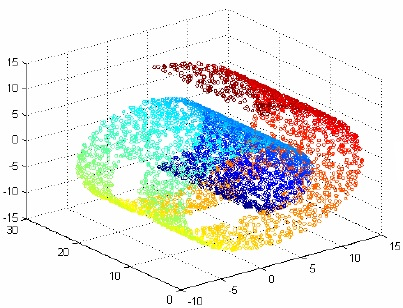
\includegraphics[width=50mm]{swissroll}
	\caption{2D 'Swiss Roll' Manifold in 3D Euclidean Space}
	\label{fig:swiss-roll}
\end{figure}

\begin{figure}[ht!]
	\centering
	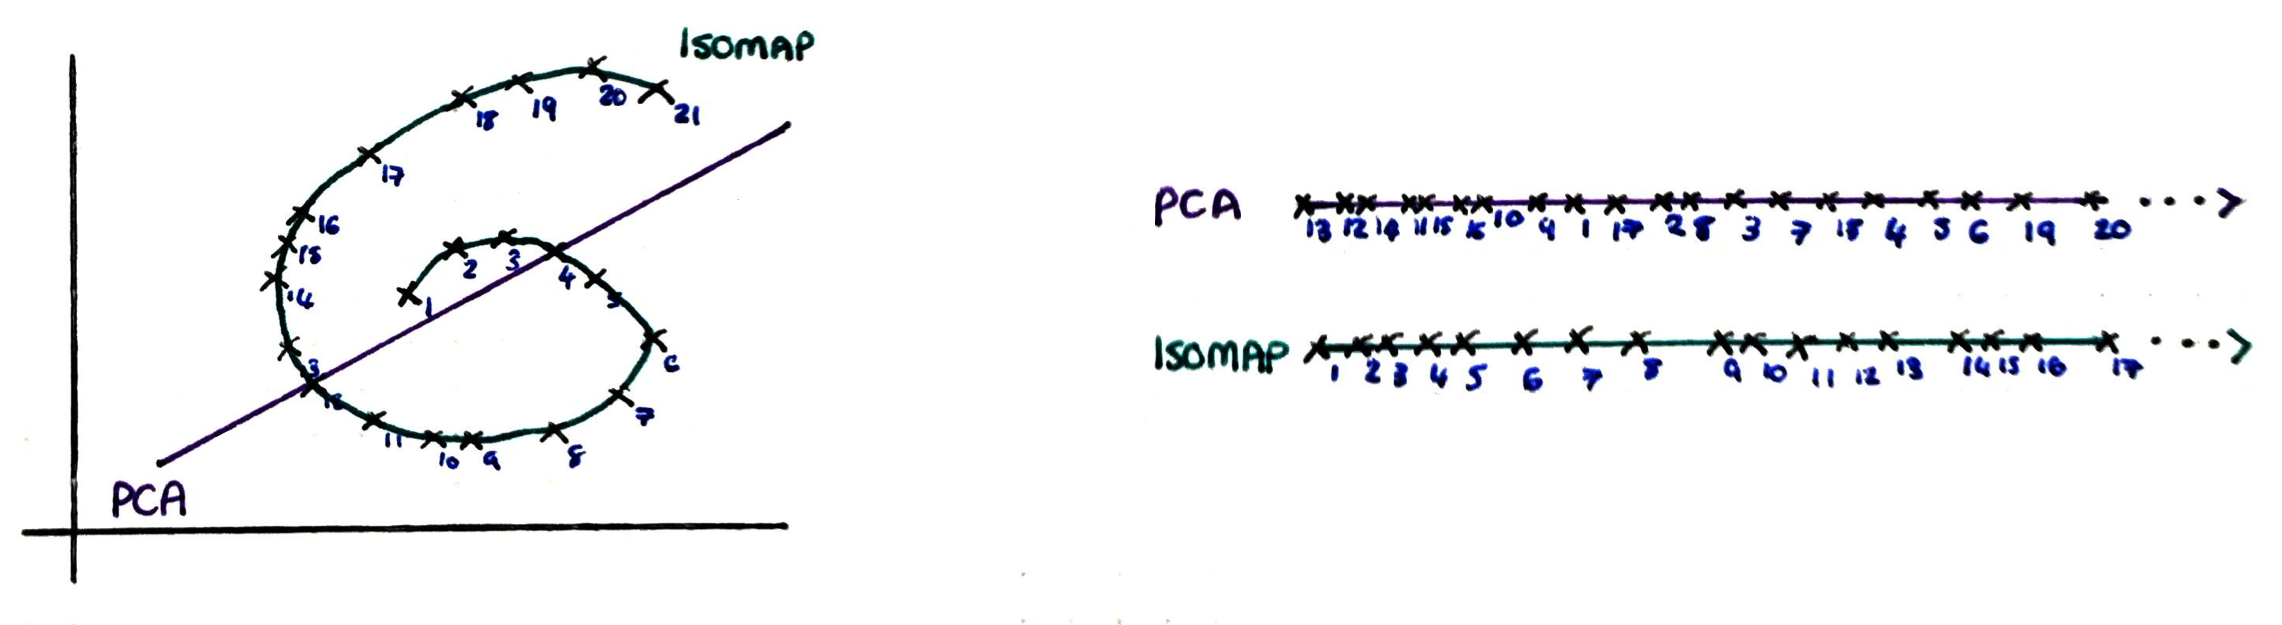
\includegraphics[width=150mm]{isomap}
	\caption{Linear (PCA) vs. Non-Linear (isomap) Dimensionality Reduction}
	\label{fig:isomap}
\end{figure}

\begin{figure}[!ht]
	\begin{subfigure}{.5\textwidth}
	\centering
	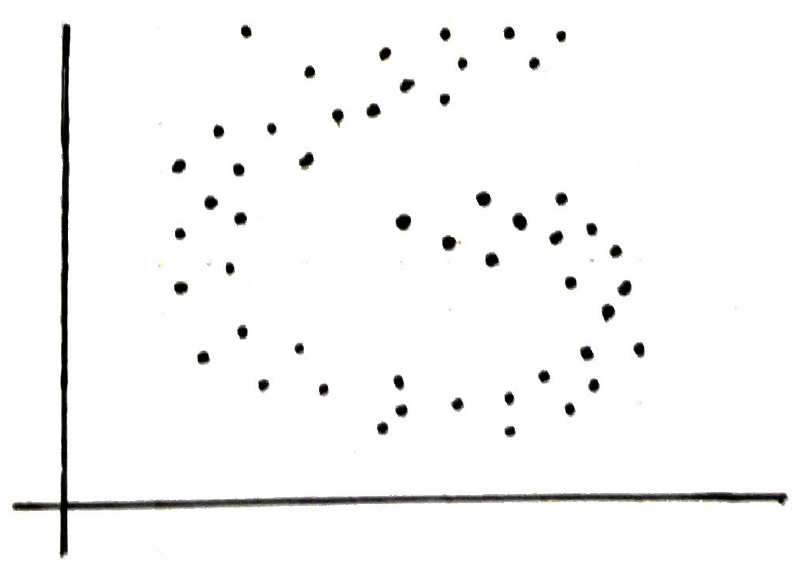
\includegraphics[width=75mm]{dpg-manifold}
	\caption{1D 'Swiss Roll' manifold in 2D Euclidean Space}
	\label{fig:manifold}
	\end{subfigure}
	\begin{subfigure}{.5\textwidth}
	\centering
	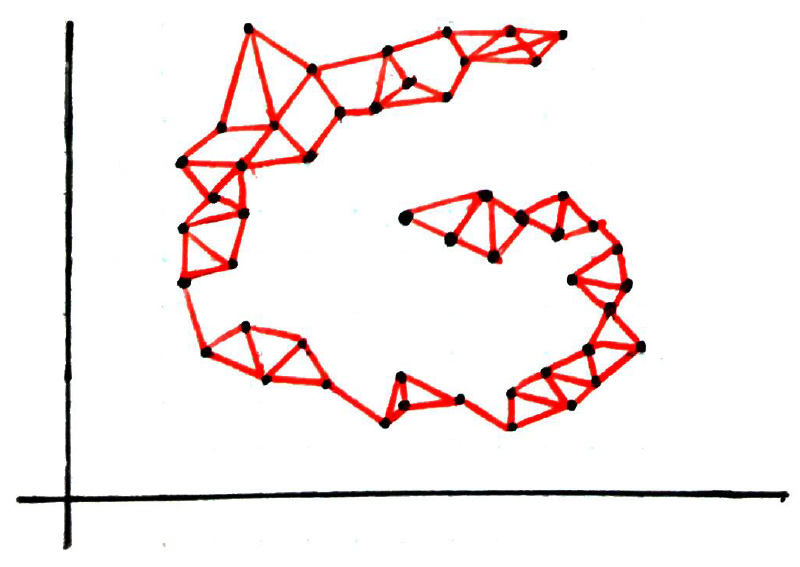
\includegraphics[width=75mm]{data-proximity-graph}
	\caption{k-nearest ($k = 3$) Data Proximity Graph}
	\label{fig:k-nearest-neighbours}
	\end{subfigure}
	\begin{subfigure}{.5\textwidth}
	\centering
	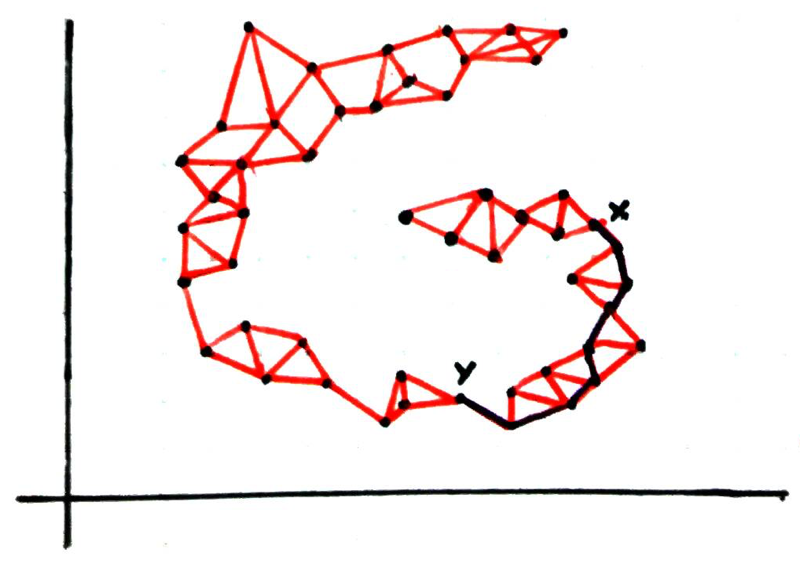
\includegraphics[width=75mm]{shortest-route}
	\caption{Shortest Route between Point $X$ and Point $Y$}
	\label{fig:route}
	\end{subfigure}
	\caption{k-nearest Neighbours ($k=3$) Data Proximity Graph for a 1D 'Swiss Roll' manifold in 2D Euclidean Space}
	\label{fig:data-proximity}
\end{figure}{}
 
\end{document}